\chapter{Introduction}
\label{cha:chapter1}

Soft robotics is a research field that evolves robots with a soft and deformable body, which guarantees them flexibility and adaptability, allowing them to face complex and unpredictable environments: for instance, they can perform smooth locomotion on rough terrain~\cite{8460667}, or squeeze through tight spaces~\cite{10.1145/2739480.2754662}

To find optimal individuals it's important to optimize both the bodies and the controllers.\\
It's clear that some individuals are intrinsically better than others at some tasks, only because of their morphology; for example, a robot with two legs surely walks better than a rigid squared box.\\
This intuitive concept is the basis of Embodied Intelligence, theory that states that the body of an agent plays a fundamental role in simplifying tasks and in making adaptive behaviours emerge through the interaction with the environment~\cite{Cianchetti2021}.\\
At the same time the controller, which is the brain telling the robot which action to take, has a key role, since it determines the behaviour of the individual in the environment.\\
For these reasons, it's important to optimize both the body and the controller of the robots, in order to find fitting morphologies with proper behaviours.

However, many existing studies focus on the controller optimization, but little attention is placed on finding the optimal bodies.
This is mainly because co-optimizing the body and the controller in robotics is characterized as a challenging problem~\cite{bhatia2021evolution}.

What makes soft robots interesting is their flexibility and softness, which makes them ideal for many future bio-related applications, since it promises an enhanced human-machine interaction.\\
They have been proposed as a support for gait rehabilitation~\cite{6696468} and colonoscopies~\cite{Zhang2019-fm}, and some other possible future applications are artificial organs and tissue-mimicking active simulators for training and biomechanical studies~\cite{Cianchetti2018}.

This work proposes soft robot co-evolution by combining two main libraries: Evolution Gym~\cite{evogym}, that provides the simulator, the co-optimization structure, the tasks to work on and an implementation of GA, and QDpy~\cite{qdpy}, for the MAP-Elites algorithm implementation, adjusted to work on soft robot evolution.

This chapter is intended to provide the basic notions of the topics related to this work, including how soft robots differ from conventional rigid robots, an overview on the algorithms used and the benchmark adopted.
The second chapter focuses on the importance of optimizing the controller, while a comparison of body optimization algorithms, MAP-Elites and GA, is proposed in the following chapter.
An analysis on how individuals behave in different environments is introduced in the fourth chapter.
Finally, the conclusions provide an overview of what emerged from the experiments presented and introduce some possible future works.


%%% SOFT ROBOTS %%%
\section{Soft Robots}
Conventionally, engineers have employed rigid materials to fabricate precise, predictable robotic systems, which are easily modelled as rigid members connected at discrete joints.\\
Rigid-bodied robots can be efficient on a single task, however they don't easily adapt to the environment.
What is more, they are often unsafe for interaction with humans.\\
A solution might be provided by soft robotics, research field that aims at evolving robots with a deformable structure and muscle-like actuation that emulates biological systems, yielding to adaptability and a smooth interaction with the environment~\cite{Rus2015}.

The body of each robot in Evolution Gym is composed of various types of primitive building blocks, and the control of the robot includes action signals applied on the actuator voxels.


\subsection{Body}
The soft robot evolved in this work are voxel-based, which means they are composed of primitive blocks of various type.
This multi-material voxel-based structure provides a general
and universal representation for various categories of robot designs, and at the same time results in a modular and expressive structure design space~\cite{bhatia2021evolution}.

The robot body is defined as a matrix, where each entry is an integer corresponding to a voxel type, defined in Table \ref{tab:voxel}, and a list of connections, describing the adjacent voxels. The bodies of the robots considered in this work are defined by a 5x5 matrix.
Note that a generated body is considered valid if it is connected and it has at least one actuator.

\begin{table}[h]
    \centering
    \begin{tabular}{|l|c|l|l|}
        \hline
        \textbf{Voxel type} & \textbf{Value} & \textbf{Color} & \textbf{Behaviour}\\
        \hline
        Empty & 0 & white & -\\
        Rigid & 1 & black & not deformable\\
        Soft & 2 & grey & deformable\\
        Horizontal actuator & 3 & orange & can expand/contract horizontally\\
        Vertical actuator & 4 & blue & can expand/contract vertically\\
        Fixed & 5 & black & not deformable, fixed position\\
        \hline
    \end{tabular}
    \caption{Voxel types representation}
    \label{tab:voxel}
\end{table}

Soft voxels are deformable under the action of external forces; actuators are the ones that allow the body motion thanks to their gradual expansion/contraction in one direction, according to the action provided by the controller.
No robot can be composed of fixed voxels, since they are only used in the definition of the environments to build, for example, the terrain to walk on.

The simulation converts all objects into a set of point masses and springs by turning each voxel
into a cross-braced square as shown in the blue panel of Figure \ref{fig:obj_repr}. The figure also displays the voxel graphic representations, together with a legend of the colors chosen to differentiate the voxels types.

\begin{figure}
    \centering
    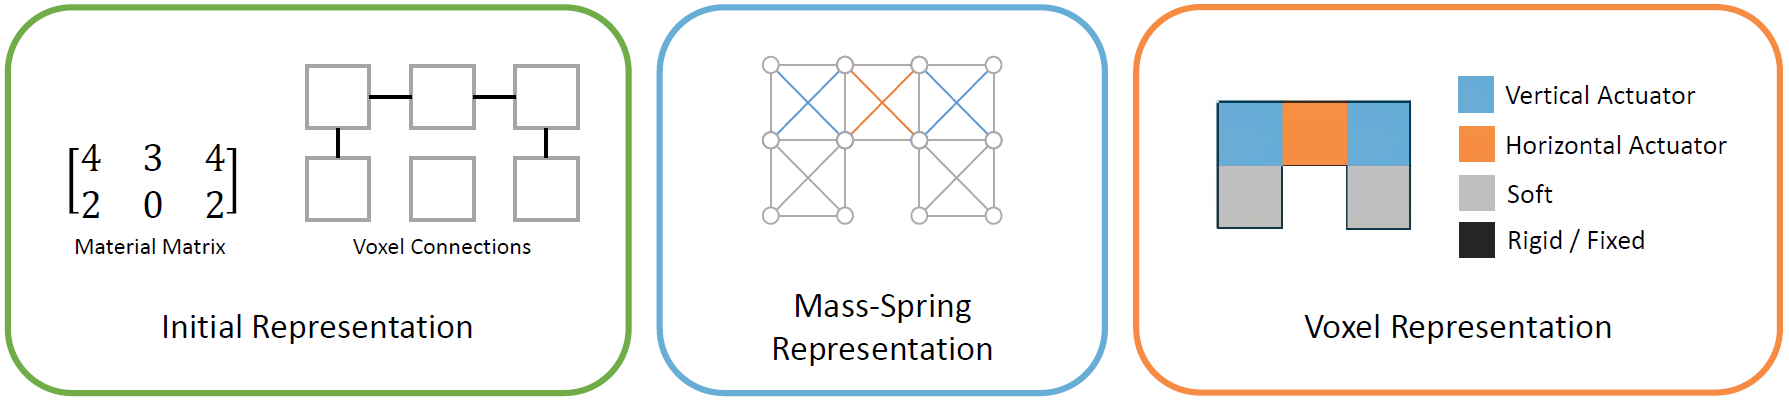
\includegraphics[scale=0.4]{images/obj_representation}
    \caption{Representation of the simulation object\cite{bhatia2021evolution}}
    \label{fig:obj_repr}
\end{figure}


\subsection{Controller}
The controller is implemented as a neural network.
It takes in input the state of the task, including observations about the robot, the environment and other task-specific information. Details about the observation space of the tasks studied in this work are provided later in this chapter.\\
The output provided by the controller is the action, a vector with length $a^r$, where $a^r$ is the number of actuators in the design of robot $r$. The action vector defines, for each actuator, its contraction/expansion value in relation to its rest length, and can vary in the range $[0.6, 1.6]$.


%%% OPTIMIZATION %%%
\section{Optimization}
Co-optimization plays a fundamental role in soft robot evolution: it's important to focus on both the body and the controller, since they both equally contribute to the performance of an individual.\\
In this work, the co-optimization applied is the one proposed by Evolution Gym, and is formulated as a two-level optimization problem~\cite{bhatia2021evolution}.\\
As shown in Figure \ref{fig:optimization}, the controller is optimized using reinforcement learning during the task simulations, and the final reward can be used by the design algorithm to determine the next morphology to work on.

As for the implementation, the design optimization is defined in the outer loop, while the inner loop focuses on control optimization, as shown in Algorithm \ref{alg:co_optimization}.\\
In this work, the controller is optimized using a reinforcement learning algorithm, PPO~\cite{kostrikov2018}, while the design optimization algorithms applied are the genetic algorithm~\cite{evogym} and MAP-Elites~\cite{qdpy}.

\begin{figure}[h]
    \centering
    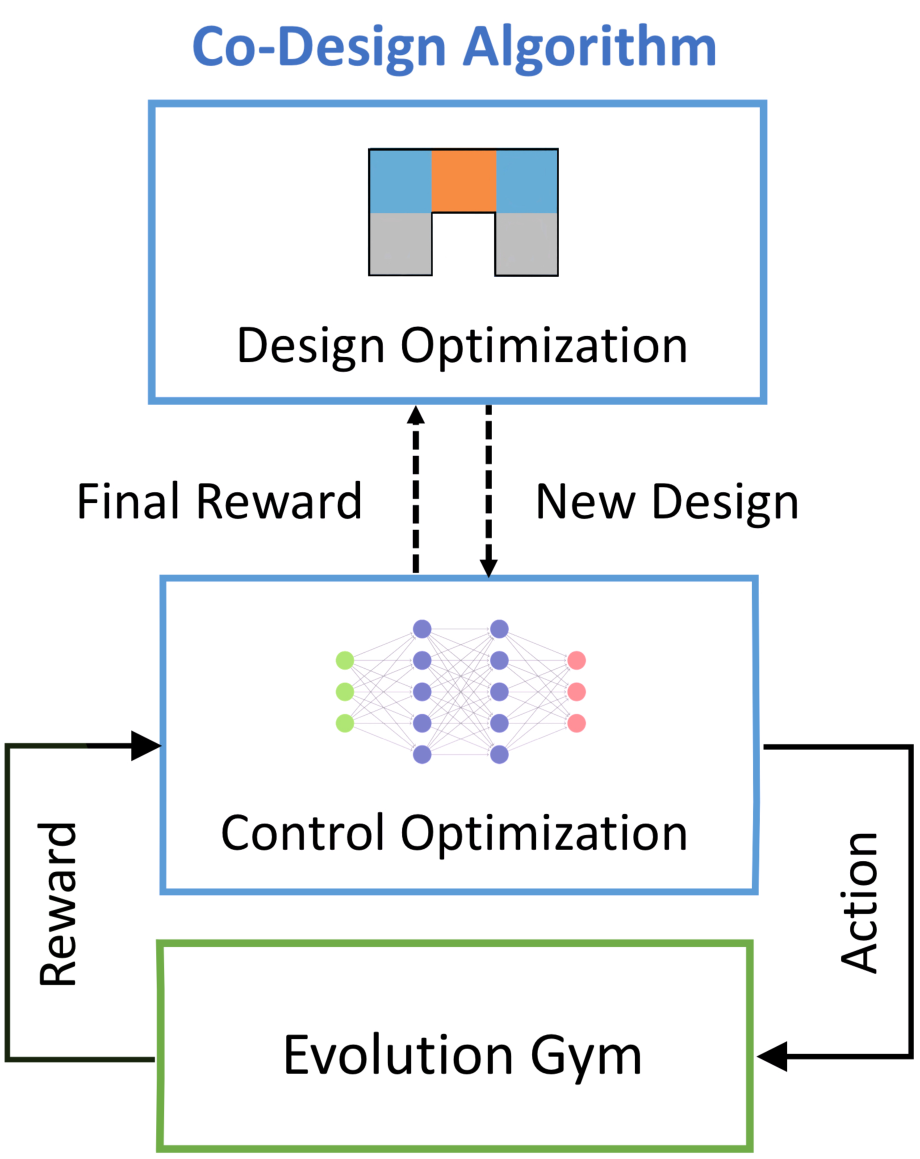
\includegraphics[scale=0.35]{images/experiment_design.pdf}
    \caption{General structure of the experiments~\cite{bhatia2021evolution}. The co-design process generates the individuals to evaluate. Evolution Gym runs the simulations according to the given bodies and controllers, and computes the reward.}
    \label{fig:optimization}
\end{figure}

\begin{algorithm}[h]
    \caption{Robot evolution co-optimization algorithm \cite{bhatia2021evolution}} \label{alg:co_optimization}
    \begin{algorithmic}
    \Require Task specification $T$, number of generations $n$, population size $p$.
        \State $S \gets \emptyset$ \hfill // Dataset of robot designs, controllers and rewards
        \State $D_1, ..., D_n \gets SampleDesigns(p)$ \hfill // Sample an initial population of robot designs
        \For{$i \gets 1$ \textbf{to} $n$}
            \For{$j \gets 1$ \textbf{to} $p$}
            \State $C_j \gets OptimizeControl(T, D_j)$ \hfill // Optimize the controller of given robot design
            \State $r_j \gets EvaluateReward(T, D_j, C_j)$ \hfill // Evaluate the reward of given design and controller
            \State $S \gets S \cup \{(D_j, C_j, r_j)\}$ \hfill // Update the evaluation result to the dataset
            \EndFor
        \State $D_1, ..., D_n \gets OptimizeDesigns(S, p)$ \hfill // Optimize a population of robot designs to evaluate
        \EndFor
    \end{algorithmic}
\end{algorithm}


\subsection{Evolutionary Algorithms}
Mainstream artificial intelligence has been very successful at designing algorithms and devices that solved stable problems. But, in doing so, in ended up neglecting fundamental aspects of biological intelligence, such as physical embodiment, behavioral autonomy, evolution and learning, that make biological organisms prone to errors and sometimes difficult to predict, but also so successful to survive in unknown and changing environments~\cite{Floreano2008}.

These premises lay out the grounding assumptions on which are founded Evolutionary Algorithms (EA): solving dynamic problems, like learning in unpredictably changing environments, requires equally dynamic solutions, that might be already provided in biology.

There are many types of EA, but the common underlying idea behind all these techniques is the same: given a population of individuals within some environment that has limited resources, competition for those resources causes natural selection (survival of the fittest)~\cite{Eiben2015}.

Applying EA to soft robot evolution has proven to be advantageous for the potential to uncover unconventional designs, difficult to anticipate for a human expert, guaranteeing efficiency and robustness.
Furthermore, evolution is able to exploit synergistic effects between body and brain that, are often too hard to model analytically.~\cite{10.1007/978-3-030-72699-7_14}

In this work two EA, introduced in the next paragraphs, are applied to soft robot design optimization: the Genetic Algorithm (GA) and the Multi-dimensional Archive of Phenotypic Elites (MAP-Elites).


\subsubsection{Genetic Algorithm}
The Genetic Algorithm (GA) is an iterative search algorithm that draws inspiration from Charles Darwin's Theory of natural selection. According to this algorithm, only the fittest individuals survive through generations. Mutation and crossover can be applied to the survivors, so as to generate offspring with more chance to fit.

The structure upon which GA are built is the following.
In each generation, the population is composed by $pop\_size$ individuals. In the first generation the designs are sampled. After the controller optimization and the evaluation, the top $x\%$  of individuals survive, and take part to the next generation. 
The survivors are iteratively sampled, and their variation, applying mutation and crossover, generates new individuals to evaluate.\\
This iterative process goes on until it meets the termination condition; in this work, the process ends when $max\_evaluations$ individuals have been evaluated.

The mutation strategy here applied states that given a morphology shape, each cell has a certain probability of mutating, defined by the \textit{mutation\_rate} parameter.
Each voxel can mutate its type into any of the others with the same probability, except for the empty type: it's three times more likely to become empty, since mutating a voxel from/to empty allows a change in the morphology. In the implementation used, no crossover has been applied.

The obtained body is considered valid if it satisfies the body constraint (being connected and having one actuator at least) and has not been already evaluated.
When the proposed body doesn't satisfy these constraints, a new mutation on the same starting individual is proposed, until the maximum number of allowed attempts, \textit{num\_attempts}, is reached.

If no valid mutated individual is found after the maximum number of attempts, it is discarded and a new body among the survivors is selected to mutate.\\


\subsubsection{MAP-Elites}
In Evolutionary Robotics a population of solutions is evolved to optimize robots that solve a given task. However, in traditional Evolutionary Algorithms, the population of solutions
tends to converge to local optima when the problem is complex or the search space is large, a problem known as premature convergence. Quality Diversity algorithms try to overcome premature convergence \cite{nordmoen2020quality} by encouraging diversity and domain illumination.

An example of QD algorithm is the Multi-dimensional Archive of Phenotypic Elites (MAP-Elites).\\
This algorithm builds a grid, where each dimension consists of a discretization of the chosen features in their domain space, according to the defined $map\_shape$.
Given the discretization, MAP-Elites searches for the highest performing solution for each cell in the N-dimensional feature space\cite{mapelites}, where N is the number of features.
Each individual is mapped to one bin only, according to its features value.
After an individual is evaluated and its features are computed, it can be inserted to the map if the corresponding bin is empty or its fitness value is greater than the one already stored, which is the occupant elite.

In the first generation, $num\_init$ individuals with randomly generated bodies are sampled, to firstly explore the map. The later generation is composed of $num\_mutated$ individuals, obtained by a mutation of bodies already evaluated and stored in the current map.\\
Individuals are evaluated in batches of size $batch\_size$.
At the end of each batch, the individuals evaluated can be inserted in the map or disregarded, as previously described.\\
The new individuals to evaluate in the next batch are generated by mutating the ones currently stored in the map.
The mutation strategy applied to these experiments is the same one used on GA, described in the previous section.\\
Note that all evaluated individuals have different morphologies since, during the experiments, evaluated bodies are hashed and stored, so as to avoid duplicated evaluations.

When all individuals are evaluated, the map represents the best individuals for each combination of features, and diversity is promoted, since different cells map to individuals with different feature values.

The features implemented and used in this work are the actuation and the emptiness of the body, described in detail in the following paragraphs.

\paragraph{Actuation}
Since Evolution Gym allows the distinction of voxel types, it's possible to define a feature that considers the number of actuators, which allow the robot motion.\\
The actuation $A$ used in these experiments is defined as follows:
\[A^r = \dfrac{a^r_v + a^r_h}{n^r}\]
where $r$ is the individual on which the feature is computed, $a_v$ and $a_h$ are  the number of vertical and horizontal actuators, and $n$ is the number of (non-empty) voxels composing the morphology.
Its domain is $[0, 1]$: when morphologies are composed by actuators only, the feature value is 1, and reducing the number of actuators makes this value tend to 0. However, actuation cannot be precisely 0, since having at least one actuator is one of the constraints to create a valid body.

\paragraph{Emptiness}
The emptiness $E$ of a robot $r$ considers the number empty cells in the robot morphology, that is the number of potential, but unused, voxels.\\
Let $e$ be the number of cells of zero value in the 2D robot body matrix (i.e. the empty voxels) and $s$ the maximum number of voxels to fill the matrix, according to the shape definition of individual $r$: 
\[E^r = \dfrac{e^r}{s^r}\]
The domain for this feature is $[0, 1]$: individuals with an emptiness value close to 1 are composed by few voxels; when emptiness is 0, it means that the body is composed by the maximum number of voxels possible.\\
Since the robots evolved in this work are defined by a 5x5 matrix, their maximum number of voxels is 25.


\subsection{Reinforcement Learning}
Reinforcement Learning (RL) is a Machine Learning paradigm that aims at mapping situations into actions.\\
The learner tries actions and gets a numerical reward, positive or negative, according to its performance on the task considered.
Thanks to the feedback derived from its interactions with the environment, good behaviours are encouraged and bad performing actions are penalized, taking to long-term results.
This trial and error method allows the agent to learn from its own experience, directly interacting with the environment.

The robot controller optimization proposed by Evolution Gym is based on the Proximal Policy Optimization (PPO), a RL algorithm which alternates between sampling data through interaction with the environment, and optimizing a “surrogate” objective function \cite{schulman2017proximal}.
PPO is an on-policy algorithm, which means that it considers a batch of data using the current policy to evaluate its reward.
Its implementation, provided by \cite{kostrikov2018}, together with the hyperparameters, has been applied to the experiments introduced in this work.


\subsection{Tasks}
Evolution Gym proposes many tasks, classified into different difficulty levels according to the performance of the baseline algorithms that were tested on them. Each environment has it's own definition of reward.
This work focused on three tasks, categorized as \textit{easy} ones: walker, pusher, carrier.

The observation space of the tasks consider parameters regarding the robot or the eventual object it interacts with.
Let $o$ be the object considered, the following are defined:
\begin{itemize}
    \item Velocity of the center of mass: $v^o$\\
        2-D vector computed averaging the velocities of all point masses composing $o$; $v^o_x$ and $v^o_y$ are the components on the $x$ and $y$ directions.
    \item Position of the center of mass: $p^o$\\
        2-D vector computed averaging the positions of all point masses composing $o$; $p^o_x$ and $p^o_y$ are the components on the $x$ and $y$ directions.
    \item Number of point masses: $n$\\
        number of point masses in the object considered.
    \item Position of all point masses: $c^o$\\
        vector of length $2n$ representing the position of all $n$ point masses of object $o$, relatively to $p^o$, the center of mass of the object.
\end{itemize}


\subsubsection{Walker-v0}
This task is the most commonly studied in soft robot evolution.
The environment is composed by a simple rigid flat terrain, and the goal of the individual is to walk as far as possible.\\
The robot $r$ is given a reward $R$ for moving in the positive x-direction:
\[R = \Delta p^r_x\]
Once it reaches the end of the terrain, it gets an additional one-time reward of 1.\\
The observation space has dimension $S \in R ^{2n+2}$, and is formed by concatenating vectors $v^r$, $c^r$, with lengths 2 and $2n$ respectively.

\begin{figure}[H]
    \centering
    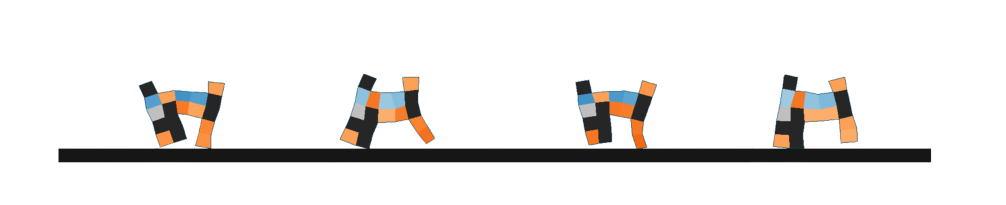
\includegraphics[scale=0.9]{images/task_walker.pdf}
    \caption{Walker-v0}
    \label{fig:task_walker}
\end{figure}


\subsubsection{Pusher-v0}
In this task the goal of the robot is to push a box initialized in front of it as far as possible.\\
The reward is $R = R_1 + R_2$, where $R_1$ is the score obtained according to the positive x direction motion of both the robot and the box, giving more importance to the latter one:
\[R_1 = 0.5 \cdot \Delta p^r_x + 0.75 \cdot \Delta p^b_x\]
$R_2$ is the penalty applied according to the separation on the x direction of the two objects:
\[R_2 = -\Delta |p^b_x - p^r_x|\]
The only components that contribute to the reward are $p^r_x$ and $p^b_x$, which are the x-direction components of the position vector $p$ of the center of mass of the robot and the box, respectively.\\
The first time the robot successfully reaches the end of the terrain, it gets a reward of 1.\\
The observation space has dimension $S \in R^{2n+6}$, and is formed by concatenating vectors $v^r$, $p^b - p^r$, $v^b$, $c^r$, with lengths 2, 2, 2, $2n$ respectively.

\begin{figure}[H]
    \centering
    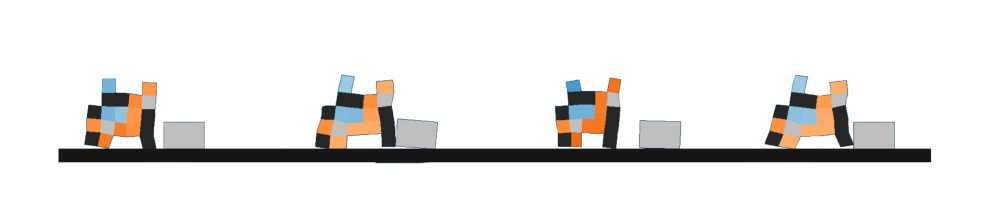
\includegraphics[scale=0.9]{images/task_pusher.pdf}
    \caption{Pusher-v0}
    \label{fig:task_pusher}
\end{figure}


\subsubsection{Carrier-v0}
The goal in this task is to carry a box, initialized above the individual, as far as possible.\\
The reward is $R = R_1 + R_2$, where $R_1$ is the score obtained according to the positive x direction motion of both the robot $r$ and the box $b$, and $R_2$ is a penalty applied when when the box falls below a certain height:
\[R_1 = 0.5 \cdot \Delta p^r_x + 0.5 \cdot \Delta p^b_x\]

\[R_2 =\begin{cases}
        0 & \text{if } p^b_y \geq t_y\\
        10 \cdot \Delta p^b_y & \text{otherwise}
    \end{cases}
    \]
where $t_y$ is the height threshold to determine whether to apply the penalty.\\
Just as in the other tasks described, the robot gets a one-time reward of 1 for successfully reaching the end of the terrain.\\
The observation space has dimension $S \in R^{2n+6}$, and is formed by concatenating vectors $v^r$, $p^b - p^r$, $v^b$, $c^r$, with lengths 2, 2, 2, $2n$ respectively.

\begin{figure}[H]
    \centering
    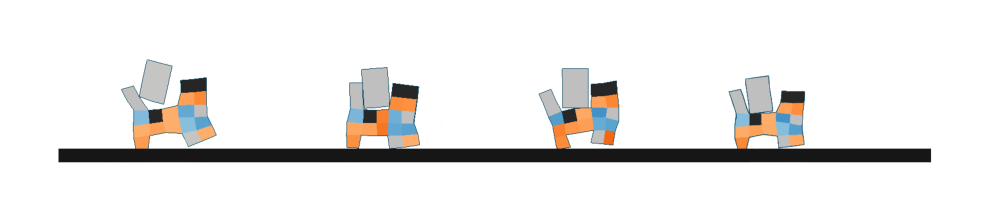
\includegraphics[scale=0.9]{images/task_carrier.pdf}
    \caption{Carrier-v0}
    \label{fig:task_carrier}
\end{figure}

\newpage